% Figure 3.7: SCORM 2004 CAM Manifest Extensions
\begin{chapterfigurebox}
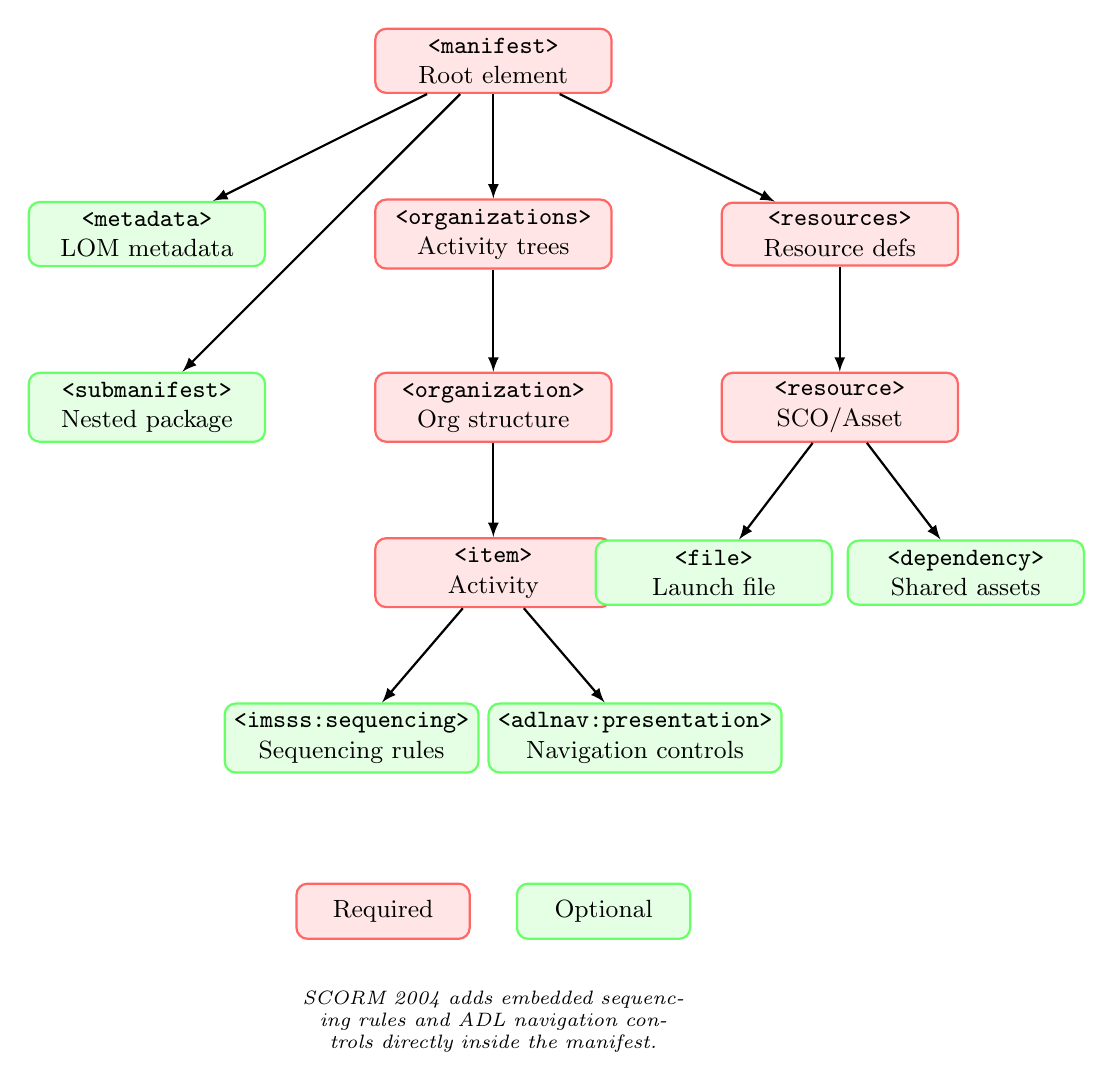
\begin{tikzpicture}[
    every node/.style={font=\small},
    arrow/.style={->, >=latex, thick},
    required/.style={rectangle, draw=red!60, fill=red!10, thick, minimum width=3cm, minimum height=0.7cm, align=center, rounded corners},
    optional/.style={rectangle, draw=green!60, fill=green!10, thick, minimum width=3cm, minimum height=0.7cm, align=center, rounded corners}
]

\node[required] (manifest) at (0,0) {\texttt{<\ENG{manifest}>}\\\ENG{Root} \ENG{element}};

\node[optional] (metadata) at (-4.4,-2.2) {\texttt{<\ENG{metadata}>}\\\ENG{LOM} \ENG{metadata}};
\node[required] (organizations) at (0,-2.2) {\texttt{<\ENG{organizations}>}\\\ENG{Activity} \ENG{trees}};
\node[required] (resources) at (4.4,-2.2) {\texttt{<\ENG{resources}>}\\\ENG{Resource} \ENG{defs}};

\node[optional] (submanifest) at (-4.4,-4.4) {\texttt{<\ENG{submanifest}>}\\\ENG{Nested} \ENG{package}};
\node[required] (org) at (0,-4.4) {\texttt{<\ENG{organization}>}\\\ENG{Org} \ENG{structure}};
\node[required] (resource) at (4.4,-4.4) {\texttt{<\ENG{resource}>}\\\ENG{SCO/Asset}};

\node[required] (item) at (0,-6.5) {\texttt{<\ENG{item}>}\\\ENG{Activity}};
\node[optional] (file) at (2.8,-6.5) {\texttt{<\ENG{file}>}\\\ENG{Launch} \ENG{file}};
\node[optional] (dependency) at (6.0,-6.5) {\texttt{<\ENG{dependency}>}\\\ENG{Shared} \ENG{assets}};

\node[optional] (sequencing) at (-1.8,-8.6) {\texttt{<\ENG{imsss:sequencing}>}\\\ENG{Sequencing} \ENG{rules}};
\node[optional] (presentation) at (1.8,-8.6) {\texttt{<\ENG{adlnav:presentation}>}\\\ENG{Navigation} \ENG{controls}};

\draw[arrow] (manifest) -- (metadata);
\draw[arrow] (manifest) -- (organizations);
\draw[arrow] (manifest) -- (resources);
\draw[arrow] (manifest) -- (submanifest);
\draw[arrow] (organizations) -- (org);
\draw[arrow] (org) -- (item);
\draw[arrow] (item) -- (sequencing);
\draw[arrow] (item) -- (presentation);
\draw[arrow] (resources) -- (resource);
\draw[arrow] (resource) -- (file);
\draw[arrow] (resource) -- (dependency);

\node[required, minimum width=2.2cm] (leg_req) at (-1.4,-10.8) {\ENG{Required}};
\node[optional, minimum width=2.2cm] (leg_opt) at (1.4,-10.8) {\ENG{Optional}};
\node[font=\scriptsize\itshape, text width=6.3cm, align=center] at (0,-12.2) {\ENG{SCORM} 2004 \ENG{adds} \ENG{embedded} \ENG{sequencing} \ENG{rules} \ENG{and} \ENG{ADL} \ENG{navigation} \ENG{controls} \ENG{directly} \ENG{inside} \ENG{the} \ENG{manifest}.};

\end{tikzpicture}
\end{chapterfigurebox}
